\documentclass[review]{elsarticle}

%\documentclass[1p,review]{elsarticle}
\usepackage{pifont}
\usepackage{booktabs}
\usepackage{natbib}
\usepackage{blkarray}
\usepackage{caption} 
\usepackage{multirow}
\usepackage{graphicx}
\usepackage{float}
\usepackage{amsmath}%
\usepackage{amsfonts}%
\usepackage{amssymb}%
\usepackage{graphicx}
\usepackage{pdflscape}
\usepackage{tablefootnote}
\usepackage{array}
\usepackage{framed}
\usepackage{setspace}
\usepackage[margin=2.5cm]{geometry}
\usepackage{graphicx}
\usepackage{caption}
\usepackage{subcaption}
\usepackage{natbib}
\usepackage{bibentry}
\usepackage{blkarray}
\usepackage{caption} 
\usepackage{multirow}
\usepackage{graphicx}
\usepackage{float}
\usepackage{amsmath}%
\usepackage{amsfonts}%
\usepackage{amssymb}%
\usepackage{tablefootnote}
\usepackage{array}
\usepackage{setspace}
\usepackage[mathlines]{lineno}
\usepackage{geometry}
\usepackage{url}
%\usepackage{subcaption}
%\usepackage{pdflscape}
\usepackage{lineno}
\usepackage{xargs}
\usepackage{amsthm}
\usepackage{graphics}
\usepackage[usenames,dvipsnames]{color}
\usepackage{enumerate}
\usepackage{dsfont}
\usepackage{tabularx}
\usepackage{tikz}\usetikzlibrary{shapes,arrows,positioning,calc,fit}



%%%%% BEGIN MIKE'S COMMANDS %%%%%
\usepackage[normalem]{ulem}  %provides strikeout \sout{}
\usepackage{xspace} %%needed for mike's commands

\newcommand\mymarginpar[1]{\marginpar{\begin{spacing}{0.7}\singlespacing \tiny #1 \end{spacing}}}  %for notes in margin

%%custom commands for sanity
\newcommand{\imax}{\ensuremath{i_{\max}}\xspace}
\newcommand{\mvec}{\ensuremath{\vec{m}}\xspace}
\newcommand{\mstarvec}{\ensuremath{\vec{m}}\xspace}
\newcommand{\GCD}{\ensuremath{\text{GCD}}\xspace}
\newcommand{\detA[1]}{\ensuremath{\ensuremath{\det\left[\bs{A}_{#1}\right]}\xspace}}

\doublespacing


%%%%% END MIKE'S COMMANDS %%%%%




%----------------------------------------------------------
\biboptions{round,authoryear}
\AtBeginDocument{\renewcommand{\bibname}{References}}
\renewcommand{\floatpagefraction}{0.1}
\newcolumntype{L}[1]{>{\raggedright\let\newline\\\arraybackslash\hspace{0pt}}m{#1}}
\newcolumntype{C}[1]{>{\centering\let\newline\\\arraybackslash\hspace{0pt}}m{#1}}
\newcolumntype{R}[1]{>{\raggedleft\let\newline\\\arraybackslash\hspace{0pt}}m{#1}}
\floatstyle{plaintop}
\restylefloat{table}
\restylefloat{figure}

%Quicklimit
\newcommand\limf[1]{\lim_{#1 \to \infty}}
%quick partials
\newcommand\p[2]{\frac{\partial #1}{\partial #2}}
\newcommand\ptwo[2]{\frac{\partial^2 #1}{\partial #2^2}}
\newcommand\mptwo[3]{\frac{\partial^2 #1}{\partial #2 \partial #3}}
%var text
\newcommand{\var}{\mathrm{var}}
%indicator
\newcommand\ind[1]{\mathds{1}_{\{#1\}}}
\newcommandx{\iton}[3][1=i,2=1,3=n]{_{#1 = #2}^{#3}}
%Norm Distrubtion
\newcommand\isnorm{\sim N(\gm,\gs^{2})}
\newcommand\issnorm{\sim N(0,1)}
\newcommand\isnormd[2]{\sim N(#1,#2)}
\newcommand\isbeta{\sim Beta(\alpha,\beta)}
\newcommand\isbetad[2]{\sim Beta(#1,#2)}
%----
\newcolumntype{A}{ >{$} r <{$} @{} >{${}} l <{$} } % A for "align"
%% (1) "r" column in math mode:          >{$} r <{$}
%% (2) no space:                         @{}
%% (3) "l" column in math mode, with 
%%     an empty subformula at the start: >{${}} l <{$}


%----


%\captionsetup[table]{skip=10pt}
%\setlength\belowcaptionskip{5pt}
\renewcommand{\arraystretch}{1.5}
\newtheorem{acknowledgement}{Acknowledgement}
\newtheorem{algorithm}{Algorithm}
\newtheorem{axiom}{Axiom}
\newtheorem{case}{Case}
\newtheorem{claim}{Claim}
\newtheorem{conclusion}{Conclusion}
\newtheorem{condition}{Condition}
\newtheorem{conjecture}{Conjecture}
\newtheorem{corollary}{Corollary}
\newtheorem{criterion}{Criterion}
\newtheorem{definition}{Definition}
\newtheorem{example}{Example}
\newtheorem{exercise}{Exercise}
\newtheorem{lemma}{Lemma}
\newtheorem{notation}{Notation}
\newtheorem{problem}{Problem}
\newtheorem{proposition}{Proposition}
\newtheorem{remark}{Remark}
\newtheorem{solution}{Solution}
\newtheorem{summary}{Summary}
\newtheorem{theorem}{Theorem}
\newtheorem{excont}{Example}
\renewcommand{\theexcont}{\theexample}
%\numberwithin{equation}{subsection}
%\numberwithin{example}{section}
\newcounter{exampleEq}
%-----------------------------------------------------------
\let\bs\boldsymbol
%----
%----
%----
\makeatletter
\@fpsep\textheight
\makeatother

%-- Flow Chart Definitions -----------------------------------------
\tikzstyle{cloud} = [rectangle, draw, fill=red!20, inner sep=0.25em, text width=5em, text centered, rounded corners, minimum height=4em, execute at begin node=\scriptsize]
\tikzstyle{subcloud} = [rectangle, draw, fill=green!20, inner sep=0.5em, text width=8em, text centered, rounded corners, minimum height=3em, execute at begin node=\scriptsize]
\tikzstyle{block} = [rectangle, draw, fill=blue!20, inner sep=0.5em, text width=13em, align=center, minimum height=3em, execute at begin node=\scriptsize]
\tikzstyle{light} = [rectangle, draw, fill=blue!10, inner sep=0.5em, text width=9em, text centered, minimum height=1em, execute at begin node=\tiny]
\tikzstyle{io} = [trapezium, draw, fill=green!20, trapezium left angle=70, trapezium right angle=-70, inner sep=0.5em, text width=5em, text centered, minimum height=3em, execute at begin node=\scriptsize]
\tikzstyle{decision} = [diamond, draw, fill=yellow!20, inner sep=0.05em, aspect=2, text width=4em, text badly centered, minimum height=5em, minimum width=7em, rounded corners, execute at begin node=\tiny]
\tikzstyle{query} = [rectangle, draw, fill=red!20, inner sep=0.5em, text width=5em, text centered, minimum height=3em, execute at begin node=\scriptsize]
\tikzstyle{prompt} = [trapezium, draw, fill=green!20, trapezium left angle=60, trapezium right angle=60, inner sep=0.5em, text width=5em, text centered, minimum height=3em, execute at begin node=\scriptsize]
\tikzstyle{stop} = [regular polygon, regular polygon sides=8, draw, fill=red!20, inner sep=0.05em, text width=5em, text centered, execute at begin node=\scriptsize]
\tikzstyle{go} = [circle, draw, fill=green!20, inner sep=0.5em, text width=5em, text centered, rounded corners, minimum height=3em, execute at begin node=\scriptsize]


\tikzstyle{line} = [draw, -latex']
\tikzstyle{noarrow} = [draw]
\tikzstyle{container} = [rectangle, draw, inner sep=0.4em, dashed, fill=none, color=red!40]



\begin{document}
\title{Modeling mRNA Populations}
\author[utkm,curradd]{N.~Pollesch\corref{cor1}}
\ead{pollesch@math.utk.edu}
\author[utkeeb,nimbios]{M.A.~Gilchrist}
\ead{mikeg@utk.edu}
\cortext[cor1]{Corresponding author}
\address[utkm]{Department of Mathematics, University of Tennessee,  Knoxville, TN 37996-1320}
\address[curradd]{Department of ??, Environmental Protection Agency, Duluth MN XXXXX}
\address[utkeeb]{Department of Ecology and Evolutionary Biology, University of Tennessee, Knoxville, TN 37996-1610}
\address[nimbios]{National Institute for Mathematical and Biological Synthesis, University of Tennessee, Knoxville, TN 37996-3410}

\begin{abstract}
This paper presents a model to describe the dynamics of protein translation.  
A system of ordinary differential equations is derived to describe the number of ribosomes bound to a strand of mRNA at a given time.
The number of ribosomes bound to an mRNA at a given time is referred to its ribosome load.
The mRNA is classified based on its ribosome load and whether or not it's marked for future degradation.  
Distribution of ribosome counts is assumed to be related to the translation initiation rate, translation completion rate, degredation marking rate, and length of the mRNA.
%The proposed marking phenomena leads to natural division of the state variables in unmarked and marked classes.
The length of the mRNA's coding region plays the role of controlling the number of ribosome counts which, in turn, determines the number of ODEs in the system.  
%This maximum number of ribosomes that can be bound at any given time as a function of gene length is denoted as \imax.
A goal of this work is to see how the equilibrium distribution between classes as changes with coding region length.
A closed form solution to the density in the $i^{th}$ ribosomal class in a system with \imax states is presented for the equilibrium distribution of the marked classes in terms of the unmarked classes.
The equilibrium solutions in the unmarked classes are shown to be related to the full determinant of the tri-diagonal matrix used to describe the system, as well as all the determinants of the minors associated to it.
In general, there is no closed form for the determinant of a tri-diagonal matrix, only a recurrence relation that can be used to find determinants.
However, in this model a closed form exists for the full determinant as it changes with changing values of \imax and its formula is presented .
This closed form for the determinant provides a method to efficiently find equilibrium solutions for the entire system.
Additionally, a continuous approximation using PDE is derived and also used to find equilibrium solutions to the system.
Both of these methods for determining equilibrium solutions are utilized in an effort to find the set of parameters that maximizes the likelihood of a given data set.
A process for mapping the equilibrium model results to data is also presented and used to begin preliminary estimation of model parameters and to verify model function.
 
\textbf{alternate abstract: Modeling Ribosomal Loading of mRNA}\\
A model is presented to describe the dynamics of protein translation related to the ribosomal load of an mRNA.
The number of ribosomes bound at a given time is referred to as ribosome load, and using this value a population of mRNA are classified.
A system of ordinary differential equations (ODEs) is derived and solved for the equilibrium distribution of a population of mRNA.
Distribution of ribosome counts is assumed to be related to the translation initiation rate, translation completion rate, degradation marking rate, and length of the mRNA.
Methods are developed to find analytical equilibrium solutions to the system of ODEs and a system of partial differential equations (PDEs) are derived to find numerical approximations to the ODE system at equilibrium as well.
Both the PDE continuous approximation and the analytical solutions to the ODE system agree offering two different methods for finding solutions at equilibrium within optimization routines.
Additionally, a tool is developed and presented that is used to compare the model results to empirical microarray data measures of ribosome load.  
\end{abstract}
\begin{keyword}
bioinformatics \sep mRNA population \sep protein translation \sep ribosome loading \sep ribosome count \sep polysome \sep mathematical model
\end{keyword}
\maketitle
%\newpage
%\tableofcontents
\newpage

\textbf{Paper Outline}
\begin{enumerate}
\item Motivation - \textbf{(Mike)}
\begin{enumerate}
\item Why is this process important?
\item What will this model enable researchers to do?
\item Other modeling efforts?
\end{enumerate}
\item Derivation and Assumptions
\begin{enumerate}
\item Physical processes captured (Ideally, have a quick discussion of process and inline definitions of variables used to represent process, followed by a total recap in a table)  - \textbf{(Nate)}
\begin{enumerate}
\item System described as population model: Dichotomy of marked and unmarked mRNA.
State variables based on an mRNA's ribosome load.
\item Process of mRNA production
\item Process of Marking mRNA for degradation supposed
\item Three processes of : Initiation, translation, and completion
%\item Originally included total number of ribosomes in system, but has since been excluded.
\end{enumerate}
\item Definition/Discussion of system boundaries - (\textbf{MIKE})
\begin{enumerate}
\item Physical boundaries as a cell and relation to parameters
\item Discussion of perceived upper and lower limits to state variables and parameters
\item Temporal boundaries and relation to steady state
\end{enumerate}
\item Assumptions: Such as initial assumptions of specific functional forms, i.e. marking rate constant among classes  - \textbf{(Nate)}
\item Justify consideration of system as two subsystems, marked and unmarked.  - \textbf{(Nate)}
\end{enumerate}
\item Model Formulation: Total model presented and then analysis of Unmarked and Marked systems  - \textbf{(Nate)}
\begin{enumerate}
\item ODE/Discrete system
\begin{enumerate}
\item Present system of ODEs (Total, Unmarked, and Marked)
\item Matrix Representation of ODE model (Total, Unmarked, and Marked)
\item Steady state formulations
%\item (Make decision to present results for steady state values for ODE here or after formulation of PDE system in a results section)
\end{enumerate}
\item PDE/Continuous system 
\begin{enumerate}
\item Explain motivation for deriving PDE
\item Explain framing as `non-linear birth and death process'
\item Explain derivation using Taylor expansion
\item Present PDE for unmarked class
\item Present non-dimensionalized system
\item Present 2nd order ODE to be solved for non-dimensionalized PDE at Equilibrium
\item Motivate and present equation for marked class at equilibrium
\item (Make decision to present results for steady state values for PDE here or in a separate section to follow)
\end{enumerate}
\end{enumerate}
\item Results  - \textbf{(Nate)}
\begin{enumerate}
\item Present solution strategies/methods
\begin{enumerate}
\item ODE/Discrete system: Matrix inversion technique
\item PDE/Continuous system: Numerical solver of 2nd order ODE that arises at equilibrium
\item Discussion of alternative solution approaches
\end{enumerate}
\item Present actual solutions for a couple sets of parameters: Highlight agreement of ODE and PDE system
\item Present solutions for discrete system under further simplifications for translation and initiation
\end{enumerate}
\item Opportunities for Future Research  - \textbf{(Nate and Mike)}
\begin{enumerate}
\item Application of model to real data.
Can highlight sources of data.
\item Alternate functional forms and relaxed assumptions
\item Further establish connection (in simplified system) to potential probability distributions
\item How to move forward with analytical solutions, specifically connection to solving 2nd order partial difference equation arising from tri-diagonal form of matrix, note here that boundary conditions exist that may be utilized which are not normally present.
\end{enumerate}
\end{enumerate}
\newpage
\section{Introduction}
This section addresses such topics as why modeling this process important, what this model will enable researchers to do, and what other modeling efforts exist that seek to achieve the same goals.

\subsection{mRNA and Translation}\label{sec:Bioligical underpinnings}
%description of the biological underpinnings of the model.
%T


\begin{enumerate}%rough ideas / poteintially important concepts
	\item Gene expression short overview
	\begin{enumerate}
		\item Gene expression is often stated as the central dogma in which genetic information encoded in the DNA is transcribed into mRNA which is subsequently translated into protein. 
		\item Often, a greater amount of attention is focused on explaining gene expression at the transcriptional level and prevailing changes of mRNA transcript levels. 
		\item However, multiple studies across all kingdoms of life have shown that transcript expression level is only moderately predictive of the final protein expression.
		\item Gene expression at the post transcriptional level is controlled by mRNA transcript stability and degradation, translation and protein maturation/degradation.
		\item The model presented in this paper encompasses gene expression regulation occuring at the translational and the mature mRNA population level.
	\end{enumerate}
	\item Biology controlling mRNA stability and translation
	\begin{enumerate}
		\item Mature mRNAs in the cytosol are called the free mRNA pool, and are in one of three states. 
		\item They are actively being translated by ribosomes and will continue to initiate new rounds of translation until the transcript is degraded.
		\item Transcripts are degraded directly from the free mRNA pool.
		\item Transcripts are protected from degradation by RNA binding protein chaperones or are found in processesing bodies awaiting translation initiation or degradation.
		\item Degradation of mature mRNAs is controlled by numerous processes depending on whether they are bound to ribosome, in processing bodies or in the free mRNA pool.
		\item Free mRNAs can be decapped or deadenylated followed by exonuclease digestion.
		\item Ribosomes can destine transcripts to degradation under multiple conditions. 
		\item The first ribosome to bind to a freshly exported transcript performs the "pioneer round of translation", which is charged with assesing the mRNA's quality.
		\item There are 3 processes which occur in the pioneer round of translation, all of which detect different mRNA defects. 
		\item No Go Decay (NGD) detects a stalled ribosome, either due to mRNA structural features, slowly translating sequence or inteference of translation elongation. %sRNA interference has been suggested, need to read sources
		\item No stop decay (NSD) detects a missing stop codon and nonsense mediated decay (NMD)  detects potential mis splicing or nonsense mutations.
		\item All three decay  mechanisms, NMD, NSD and NGD lead to the eventual degradation of their bound transcripts. 
		\item While NSD and NMD are a restricted to the pioneering round of translation, NGD can also uccur during the following rounds of translation.
		\item As transcripts are cleared by the pioneering round of translations more ribosomes can attach to the transcript, once more than one ribosome is on a transcript this ribosome mRNA complex is called a polysome.
		\item Transcripts associated to ribosomes are generally assumed to be protected from degradation and only degraded once ribosomes are off the transcript, however both NGD, (sRNA silencing) and 
			a process called cotranslational decay can degrade actively translated transcripts.
		\item Cotranslational decay involved the decapping of actively translating mRNA transcripts and subsequent 5' to 3' mRNA degradation which follows a 3 nucleotide periodic pattern in step with the Ribosome. 
	\end{enumerate}
	\item Current Models/Research and how our model fits in the current field

\end{enumerate}





\section{Model Description and Notation}\label{sec:description}
The mechanistic view that is taken for building this model is as follows.
Unbound, unmarked mRNA are introduced to the system at a constant rate of $\lambda$.
%Biologically this is representative of the addition of fully mature, translation competent mRNAs into the cytoplasmic mRNA pool.
If an unmarked mRNA has a ribosome load of 0, it is defined as being in class $m_0$ and contributes to that class's abundance.
% This is the free mRNA pool and can be found in both the cytoplasm and processing bodies awaiting tranlation initiation or degradation
Ribosomal binding to mRNA in class $i$, $m_i$, is assumed to proceed at rate $\kappa(i)$. %translation initiation
Ribosomes completing translation of the coding region are released from the mRNA at rate $\tau(i)$.  %Combination of  translation elongation and termination
mRNAs in the unmarked classes can then transition freely between the $m_0$ and $m_{\imax}$ according to initiation and completion rates until they are marked, which ultimately leads to the degradation of the mRNA.
To begin the process of mRNA degradation, marking of an mRNA in class $i$ takes place at rate of $\mu(i)$.
%Biologically $\mu$  represents different processes according to the class upon which it is acting on. 
%$\mu$ in class 0 represents deadenylationa and decapping directly.
%$\mu_1$ in class 1 can represent a multitude of processes: 1) cotranslational decay where ribosomes complete translation as depicted in the model
%2) NMD, NGD, NSD or miRNA interference where a class $m_1$ transcript falls directly to the $m_0^*$ category, goes directly to jail does not pass go and does not collect $200.
%$\mu_i>1$ is somewhat similar to class one, but has fewer biological interpretations 1) cotranslational decay where ribosomes complete translation as depicted in the model
%2) NGD or miRNA interference where a class $m_1$ transcript falls directly to the $m_0^*$ category
A marked mRNA with a ribosome load of $i$ is denoted as being in class $m_i^*$.
Once an mRNA has been marked, it is assumed that no more initiation can take place and only translation completion occurs; this completion occurs until the mRNA's ribosome load drops to 0, at which point it leaves the system from state $m_0^*$ at a constant rate of $\delta$.
%Delta is the final complete degradation of the complete decapped/deadenylated mRNA or mRNA fragments. 
%The one exception to this is cotranslation decay, where the majority of the transcript is degraded cotranslationally and only the 3' UTR and poly A tail is left following the transcript entering $m_0^*$
Figure~\ref{fig:flow_diagram} provides a diagram of system flow to accompany the description above.
Table~\ref{tab:params} provides a summary of state variable and parameter notation.

% begin flow diagram for ODE
\begin{figure} [htbp] \centering
	\begin{framed}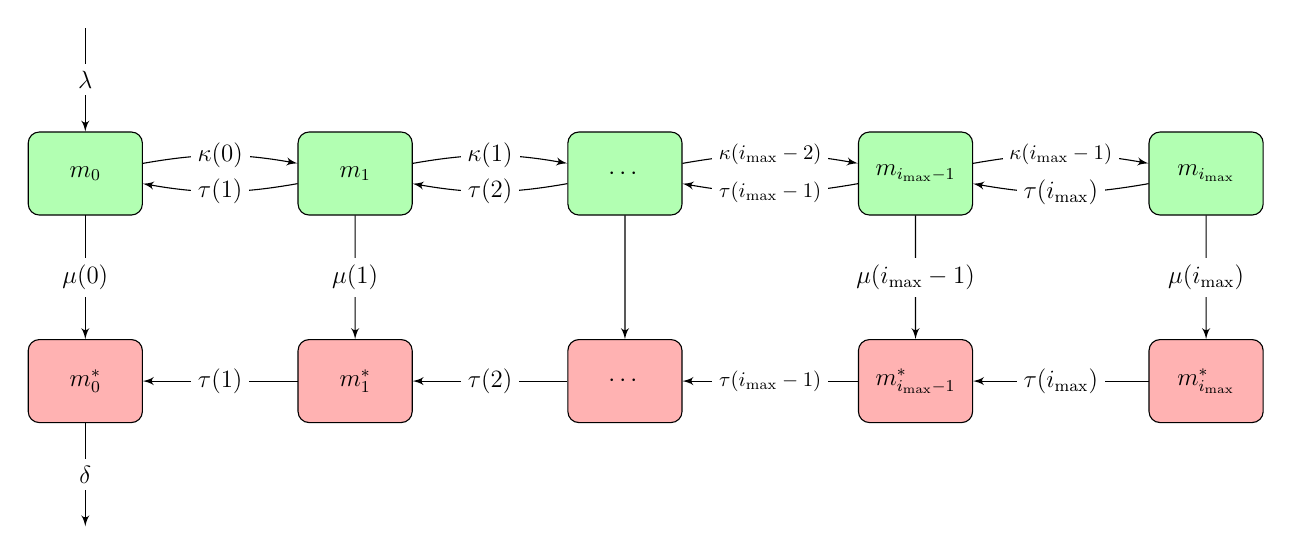
\begin{tikzpicture}[every node/.style={rectangle,fill=white,node distance=16ex, scale=0.75}, scale=0.90]
		% Row 1
		\node[cloud, fill=green!30](m0) {\large $m_0$};
		\node[cloud, fill=green!30, right of = m0, node distance = 13em](m1){\large $m_1$};
		\node[cloud, fill=green!30, right of = m1, node distance = 13em](cdots1){\large $\cdots$};
		\node[cloud, fill=green!30, right of = cdots1, node distance = 14em](mimaxn){\large $m_{\imax-1}$};
		\node[cloud, fill=green!30, right of = mimaxn, node distance = 14em](mimax){\large $m_{\imax}$};
		
		% Row 2
		\node[cloud, fill=red!30, below of = m0, node distance = 10em](m*0) {\large $m^*_0$};
		\node[cloud, fill=red!30, below of = m1, node distance = 10em](m*1){\large $m^*_1$};
		\node[cloud, fill=red!30, below of = cdots1, node distance = 10em](cdots2){\large $\cdots$};
		\node[cloud, fill=red!30, below of = mimaxn, node distance = 10em](m*imaxn){\large $m^*_{\imax-1}$};
		\node[cloud, fill=red!30, below of = mimax, node distance = 10em](m*imax){\large $m^*_{\imax}$};
		
		% empty nodes for input and output flow arrows		
		\coordinate[above of=m0, node distance=7em] (lambda);
		\coordinate[below of=m*0, node distance=7em] (delta);
		
		% Paths
		\path [line] (lambda) -- node[]{\large $\lambda$} (m0);
		\path [line] (m0) to [bend left=10] node{\large $\kappa(0)$} (m1);
		\path [line] (m1) to [bend left=10] node{\large $\kappa(1)$} (cdots1);
		\path [line] (cdots1) to [bend left=10] node{\normalsize $\kappa(\imax-2)$} (mimaxn);
		\path [line] (mimaxn) to [bend left=10] node{\normalsize $\kappa(\imax-1)$} (mimax);
		\path [line] (m1) to [bend left=10] node{\large $\tau(1)$} (m0);
		\path [line] (cdots1) to [bend left=10] node{\large $\tau(2)$} (m1);
		\path [line] (mimaxn) to [bend left=10] node{\normalsize $\tau(\imax-1)$} (cdots1);
		\path [line] (mimax) to [bend left=10] node{\large $\tau(\imax)$} (mimaxn);
		\path [line] (m0) -- node[]{\large $\mu(0)$} (m*0);
		\path [line] (m1) -- node[]{\large $\mu(1)$} (m*1);
		%Options for middle path between (...)
		\path [line] (cdots1) -- (cdots2);
		%\path [line] (cdots1) -- node[]{\large $\mu(\cdots)$} (cdots2);
		\path [line] (mimaxn) -- node[]{\large $\mu(\imax-1)$} (m*imaxn);
		\path [line] (mimax) -- node[]{\large $\mu(\imax)$} (m*imax);
		\path [line] (m*1) -- node[]{\large $\tau(1)$} (m*0);
		\path [line] (cdots2) -- node[]{\large $\tau(2)$} (m*1);
		\path [line] (m*imaxn) -- node[]{\normalsize $\tau(\imax-1)$} (cdots2);
		\path [line] (m*imax) -- node[]{\large $\tau(\imax)$} (m*imaxn);
		\path [line] (m*0) -- node[]{\large $\delta$} (delta);
		
	\end{tikzpicture}
	\caption{Flow diagram for ODE system describing transitions within the mRNA population model.
State variables and parameters are defined in Table~\ref{tab:params}.
Model description and notation are described in Section~\ref{sec:description}.}
	\label{fig:flow_diagram}
	\end{framed}
\end{figure}

\begin{table}
\centering
\begin{tabular}{|rp{4in}|}\hline
\textbf{Symbol}&\textbf{Description}\\ \hline\hline
State Variables & \\ \hline
$m_i$ & Abundance of mRNAs with a ribosome load of $i$ not marked for degradation. \\
$m_i^*$ & Abundance of mRNAs with a ribosome load of $i$ marked for degradation. \\ \hline
\multicolumn{2}{r}{Model Parameters} \\ \hline
  \imax & \shortstack{Maximum number of ribosomes able to bind to mRNA;\\
           defines number of state variables and is a function of gene length.} \\
$\kappa(i)$ & Translation initiation rate for unmarked mRNAs with a ribosome load of $i$.\\
$\tau(i)$ & Translation completion rate for the marked and unmarked mRNAs with a ribosome load of $i$. \\
$\mu(i)$ & Marking rate for unmarked mRNAs with a ribosome load of $i$.\\
$\lambda$ & Production rate of newly produced, ribosome free, and unmarked mRNA to the $m_0$ class.\\
$\delta$ & Removal rate of marked mRNA with a ribosome load of 0 from the $m_0^*$ class.\\ \hline \hline
%\multicolumn{3}{|p{450pt}|}{\footnotesize Note: $\mathbb{R}^+$ represents the non-negative real numbers and $\mathbb{Z}^{(+)}$ represents the strictly positive integers.} \\ \hline
\end{tabular}
\caption{State variables and model parameters for ODE model of mRNA populations.
Variable \imax is in the domain of non-negative integers; all other variables are non-negative real numbers.}
\label{tab:params}
\end{table}

\section{Model Definition and Analysis}
For simplicity, we begin by defining our model equations using generic functions to describe the transition of mRNAs between different classes or states.
We then constrain the model by assuming specific functions to describe the transition of mRNAs between classes.
%Note that from here forward the unmarked and marked subsystems are presented separately, the benefits of taking this approach will become evident as we proceed.  

\subsection*{General Model Equations}
%\subsection{The Unmarked subsystem}
Our model consists of two sets of time dependent and coupled ODEs.
Each set of ODEs describes the abundance of mRNAs that are either unmarked and marked for degradation.
The ODEs within each sets equations are structured by the ribosome load of the mRNA.
The coupled ODEs within a set of equations describe how mRNAs are introduced to the set, the transitions in ribosome load via initiation or completion of protein translation,  and the transition between sets either via the marking of unmarked mRNAs or the degradation of marked mRNAs with a ribosome load of 0.

Specifically, new mRNA enter the $0^{th}$ unmarked class $m_0(t)$ at a rate..
Ribosomal bind mRNAs in the $i^{th}$ unmarked class at a rate $\kappa(i)$, increasing the mRNA's ribsome load to the $i+1^{th}$ class.
By definition, $\kappa(\imax)= 0$, i.e.~mRNAs with a ribosome load of \imax cannot accommodate any addtional mRNAs.
Unmarked mRNAs with ribosome load $i$ are marked at a rate of $\mu(i)$.
Accordingly, the ribosome load of marked mRNAs remains unchanged, but they are transitioned from the unmarked class $m_i(t)$ to the marked class $m_i^*(t)$ .
Ribosome movement along an mRNA is assumed to occur independent of whether or not its unmarked or marked for degradation.
Thus, ribosomes complete translation of both marked and unmarked mRNAs with ribosome load $i$ at rate $\tau(i)$, decreasing the mRNA's ribosome load to the $i-1^{th}$ class. %class or state? State variables
Since mRNA's with a ribosome load of 0 have no ribosomes which can complete translation, by definition $\tau(0) = 0$.
Only mRNAs marked for degradation and with a ribosome load of 0 are removed from the system.
Specifically, marked mRNAs are removed from the $0^{th}$ class at a rate of $\delta m^*_0(t)$.

The functional form of the unmarked subsystem is:
\begin{align*}
\frac{dm_{0}}{dt} &= \lambda+\tau(1)m_{1}-\left(\kappa(0) + \mu(0)\right)m_{0} \\
\frac{dm_{1}}{dt} &= \kappa(0)m_{0}+\tau(2)m_{2}-\left(\tau(1)+\kappa(1)+\mu(1)\right) m_{1}\\
& \vdots & \\
\frac{dm_{i}}{dt} &= \kappa(i-1)m_{i-1}+\tau(i+1)m_{i+1}-\left(\tau(i)+\kappa(i)+\mu(i)\right) m_{i} \\
& \vdots & \\
\frac{dm_{\imax}}{dt} &= \kappa(\imax-1)m_{\imax-1}-\left(\tau(\imax)+\mu(\imax)\right) m_{\imax}\\
\end{align*}

Similarly, the functional form of the marked subsystem is:
\begin{align*}
\frac{dm_{0}^{*}}{dt} &= \mu(0)m_{0}+\tau(1)m_{1}^{*}-\delta m_{0}^{*} \\
\frac{dm_{1}^{*}}{dt} &= \mu(1)m_{1}+\tau(2)m_{2}^{*}-\tau(1)m_{1}^{*} \\
& \vdots & \\
\frac{dm_{i}^{*}}{dt} &= \mu(i)m_{i}+\tau(i+1)m_{i+1}^{*}-\tau(i)m_{i}^{*} \\
& \vdots & \\
\frac{dm_{\imax}^{*}}{dt} &= \mu(\imax)m_{\imax}^{*}-\tau(\imax)m_{\imax} \\
\end{align*}

\subsection{Model Equations Assuming Specific Transition Functions}\label{sec:assumed_forms}
As stated above, we assume mRNAs marked for degradation cannot initiate translation.
Thus the initiation function for the marked set of mRNAS is $\kappa(i) = 0$.
In contrast,  ribosomes can initiate translation on an mRNA marked for degradation.
For simplicity, we assume ribosome binding of an mRNA is independent of their ribosome load, but that successful initiation of translation is affected by ribosome load.
Specifically, we assume the start codon must be unoccupied by a ribosome in order for translation initiation to be successful.
Because we not modeling the explicit movement of ribosomes along an mRNA, we assume that at steady state probability of finding a ribosome at any given codon position within the coding sequence follows a uniform distribution.
As a consequence of this assumption, the probability of a ribosome occupying a given position on an mRNA with a ribosome load of $i$ is simply $i/\imax$.
Thus, the probability the start codon is unoccupied is $1-i/\imax$ and, in turn, our translation initiation rate function can be defined as, 
\begin{equation}\label{eq:kappa}
\kappa(i)=\kappa_0\left(1-\frac{i}{\imax}\right),
\end{equation} 
where $\kappa_0$ is a gene specific parameter that describes the rate at which unmarked mRNAs encounter and are bound by ribosomes within the cytosol (i.e.~it is an implicit function of the abundance of free ribosomes which we assume is constant).


Similarly, the probability a ribosome is at the penultimate codon (i.e.~the codon immediately upstream from the stop codon) is $i/\imax$.
Assuming that the rate of translation termination is greater than the average elongation rate (i.e.~translation termination is not a rate limiting step), we can define our translation completion rate function as,
\begin{equation}\label{eq:tau}
\tau(i)=\tau^\prime_0 i/\imax = \tau_0 i,
\end{equation}
\mymarginpar{mikeg: 10/15/19: updated $\tau$ to explicitly include $1/imax$. Earlier notes indicate this term was implicitly absorbed into $\tau_0$.
  mikeg: 10/22/19: updated to introduce $\tau^\prime_0$ and then reabsorb \imax into $\tau_0$ carrying this term through.
TODO update all later instances of $\tau_0$ with $\tau^\prime_0/\imax$ and then simplify math by canceling out \imax term and changing notation to remove the $\prime$ since it becomes unnecessary at that point.}
% \mymarginpar{Should this be $i/(\tau \imax)$?
%  On re-consideration that seems to sense since the probability a ribosome is at the final position is $1/\imax$.
%  However, I seem to recall deriving this result that indicate otherwise.
%  This shouldn't affect anything in this paper, but might explain some issues when fitting the data to model.
%  TODO for mike: Check notes.}
	%% Mike, the arguement for the derivation was as follows (if I remember correctly): For an mRNA with i ribosomes bound, it was assumed that each ribsome had an equal probability of being in any position, therefore, a ribosome was equally likely to be completing translation, therefore the probability of translation being completed was equal to the number of ribosomes bound, and thus the rate proportional to the number of ribosomes bound, leading to the form provided in eq:tau.  Does that stack up with what you were thinking?
where $\tau_0$ describes the average elongation rate of a ribosome along the protein coding sequence of that gene and, thus, could vary between genes.
Finally, we assume that unmarked mRNAs are marked for degradation rate independent of their ribosome load, i.e. $\mu(i)=\mu_0$.
As with $\tau_0$,  $\mu_0$ is assumed to fixed for a given gene, but may vary between genes.

Incorporating these explicit functional forms leads to representation of unmarked subsystem as: %\subsubsection{The Unmarked subsystem with Assumed Forms for $\kappa(i)$, $\tau(i)$, and $\mu(i)$}\label{sec:unmarked_simp}
\begin{align*}
\frac{dm_{0}}{dt} &= \lambda+\tau_0 m_{1}-\left(\kappa_0 +\mu_0\right) m_{0} \\
\frac{dm_{1}}{dt} &= \kappa_0 m_{0}+2\tau_0 m_{2}-\left(\tau_0 +\kappa_0\left(1-\frac{1}{\imax}\right) +\mu_0\right) m_{1}\\
& \vdots & \\
\frac{dm_{i}}{dt} &= \kappa_0\left(1-\frac{i-1}{\imax}\right) m_{i-1}+(i+1)\tau_0 m_{i+1}-\left(i\tau_0+\kappa_0\left(1-\frac{i}{\imax}\right) + \mu_0\right) m_{i} \\
& \vdots & \\
\frac{dm_{\imax}}{dt} &= \kappa_0\left(1-\frac{\imax-1}{\imax}\right) m_{\imax-1}-\left(\imax\tau_0 -\mu_0\right) m_{\imax} \\
\end{align*}
and the marked subsystem as,
%\subsubsection{The Marked subsystem with Assumed Forms for $\kappa(i)$, $\tau(i)$, and $\mu(i)$}\label{sec:marked_simp}
\begin{align*}
\frac{dm_{0}^{*}}{dt} &= \mu_0 m_{0}+\tau_0 m_{1}^{*}-\delta m_{0}^{*} \\
\frac{dm_{1}^{*}}{dt} &= \mu_0 m_{1}+2\tau_0 m_{2}^{*}- \tau_0 m_{1}^{*} \\
& \vdots & \\
\frac{dm_{i}^{*}}{dt} &= \mu_0 m_{i}+(i+1)\tau_0 m_{i+1}^{*}-i\tau_0m_{i}^{*} \\
& \vdots & \\
\frac{dm_{\imax}^{*}}{dt} &= \mu_0 m_{\imax}^{*}-\imax\tau_0 m_{\imax}. \\
\end{align*}
%These equations are redundant. %%% NOT ADDRESSED AS OF 8/7 
\subsection{Matrix-vector Formulation of ODE System}
It is frequently useful to work with the matrix-vector formulation for a system of ODE.
In this model, the dynamics of the marked and unmarked mRNAs can be represented as,
\begin{equation}\label{eq:matrix_full}\vec{M}'=\boldsymbol{F}\vec{M}+\vec{B},
\end{equation} 
where $\vec{M}\in\mathbb{R}^{2(\imax+1)}$ is a vector of all state variables, ordered here as $m_0$, $m_1$, ..., $m_{\imax}$, $m^*_0$, $m^*_1$, ..., $m^*_{\imax}$, $\vec{M}'$ is the vector containing the first derivatives of $\vec{M}$ with respect to time, $\bs{F}\in\mathbb{R}^{2(\imax+1)\times 2(\imax+1)}$ is the matrix representing the full system (Equation~\ref{eq:full_matrix}), and $\vec{B}\in\mathbb{R}^{2(\imax+1)}$ is the vector of $\lambda$ as the first component and 0s else.
Using the functional forms presented above, matrix formulations are provided next.

As opposed to explicitly listing elements of the full system matrix-vector representation we found that it is more convenient to utilize the block structure that emerges in this system and explicitly provide the block components.
The matrix $\bs{F}$ is block lower-diagonal and is given in Equation~\ref{eq:full_matrix}.
\begin{equation}
\label{eq:full_matrix}
\bs{F}=\left(\begin{array}{cc}
\bs{U} & \bs{0} \\
\bs{\mu} & \bs{R} \\
\end{array} \right).
\end{equation}
The upper-left block, $\bs{U}$, corresponds to the unmarked state variables, where $\bs{U}$'s general form is provided in Equation~\ref{eq:unmarked_matrix}.
The upper-right block is a matrix of all zeros, $\bs{0}\in\mathbb{R}^{\imax+1\times \imax+1}$.
Using $\bs{I}$ to represent the $\imax+1\times \imax+1$ identity matrix, the lower-left block is $\bs{\mu}=\mu_0\bs{I}$, a diagonal matrix with the constant $\mu_0$ on the diagonal and 0s else.
The lower-right block, $\bs{R}$, corresponds to the marked state variables and its form is provided in Equation~\ref{eq:marked_matrix}.

The matrix $\bs{U}$ is $(\imax+1\times \imax+1)$ dimensional and is tri-diagonal with non-zero entries on the diagonal, super-, and sub-diagonals,
\begin{equation}
\label{eq:unmarked_matrix}
\bs{U}=\left(\begin{array}{cccccc}
-(\kappa_0+\mu_0) & \tau_0 &  &  &  & \\
\kappa_0 & \left(1-\frac{1}{\imax} \kappa_0+\mu_0+\tau_0\right) & 2\tau_0 &  &  & \\
   &\ddots        & \ddots        & \ddots & &  \\
   & &    1-\frac{(i-1)}{\imax}\kappa_0 & -\left(1-\frac{i}{\imax}\kappa_0+\mu_0+i\tau_0\right) & (i+1)\tau_0 & \\
                  &         &        & \ddots  & \ddots & \ddots \\
     
                          &        &  &  & \frac{1}{\imax}\kappa_0 & -\left(\mu_0+\imax\tau_0\right) \\
\end{array}\right).
\end{equation}
In the representation given in Equation~\ref{eq:unmarked_matrix}, all blank entries are 0.
The $(\imax-1)^{\text{th}}$ row has been suppressed in Equation~\ref{eq:unmarked_matrix}, but it can be generated using the formula included for the $i^{th}$ row.

The matrix $\bs{R}$ is the lower-right block in the block lower-diagonal matrix $\bs{F}$ (Equation~\ref{eq:full_matrix}),
\begin{equation}
\label{eq:marked_matrix}
\bs{R}=\left(
\begin{array}{ccccccc}
-\delta & \tau_0 & & & & & \\
 & -\tau_0 & 2\tau_0 & & & &\\
 & & \ddots & \ddots & & & \\
 & & & -(i-1)\tau_0 & (i+1)\tau_0 & & \\
 & & & & \ddots & \ddots & \\
 & & & & & -(\imax-2)\tau_0 & \imax\tau_0 \\
 & & & & & & -\imax\tau_0 \\
\end{array}
\right),
\end{equation}
$\bs{R}$ is upper-diagonal with only non-zero entries on the diagonal and the super-diagonal.

\subsubsection{Unmarked Subsystem Matrix-vector Representation}
As a group the unmarked subsystem decouples from the marked subsystem, as such the unmarked subsystem can be solved independently of the marked subsystem.  
The matrix-vector formula representing the unmarked subsystem is \begin{equation}\label{eq:matrix_unmarked}\vec{m}'=\bs{U}\vec{m}+\vec{b},\end{equation} where $\vec{m}\in\mathbb{R}^{\imax+1}$ is the vector of unmarked state variables ordered $m_0$, ..., $m_{\imax}$, $\vec{m}'$ is the vector containing the first derivatives of $\vec{m}$ with respect to time, $\bs{U}\in\mathbb{R}^{\imax+1\times \imax+1}$ is the matrix representing the unmarked subsystem (Figure~\ref{eq:unmarked_matrix}), and $\vec{b}\in\mathbb{R}^{\imax+1}$ is the vector of $\lambda$ as the first component and 0s else.
With all equations defined for the full ODE system, include matrix-vector representations, the next section outlines methods for finding steady-state solutions to the system.



%\begin{landscape}
%\begin{figure}
%\tiny
%\centering
%\caption{Equation~\ref{eq:matrix_unmarked}, $\vec{m}'=\bs{U}\vec{m}+\vec{b}$, is the matrix-vector equation representing the unmarked system from Section~\ref{sec:unmarked_simp}. As it can be seen, the matrix $\bs{U}$ is tri-diagonal, where all blank entries appearing in the matrix are 0. This property of $\bs{U}$ is desirable and leads to a scheme for finding equilibrium solutions that is presented later in this paper}
%\label{fig:unmarked_matrix}
%\[\left(\begin{array}{c}
%m_{0}'\\
%m_{1}'\\
%\vdots\\
%m_{i}'\\
%\vdots\\
%m_{\imax-1}'\\
%m_{\imax}'
%\end{array}\right)=\left(\begin{array}{cccccccc}
%-(\kappa_0+\mu_0) & \tau_0 &  &  &  &  &  &   \\
%\kappa_0 & -\left(\frac{\imax-1}{\imax} \kappa_0+\mu_0+\tau_0\right) & 2\tau_0 &  &  &  &  &   \\
%   &\ddots        & \ddots        & \ddots & &  &  &  \\
%   & &    \frac{\imax-(i-1)}{\imax}\kappa_0 & -\left(\frac{\imax-i}{\imax}\kappa_0+\mu_0+i\tau_0\right) & (i+1)\tau_0 &  &  & \\
%                  &         &        & \ddots  & \ddots & \ddots &  &   \\
%                  &         &        &  & \frac{2}{\imax}\kappa_0 & -\left(\frac{1}{\imax}\kappa_0+\mu_0+(\imax-1)\tau_0\right) & (\imax)\tau_0 &   \\
%                          &        &  &  &  &  & \frac{1}{\imax}\kappa_0 & -\left(\mu_0+\imax\tau_0\right) \\
%\end{array}\right)\left(\begin{array}{c}
%m_{0}\\
%m_{1}\\
%\vdots\\
%m_{i}\\
%\vdots\\
%m_{\imax-1}\\
%m_{\imax}\end{array}\right)+\left(\begin{array}{c}
%\lambda\\
%0\\
%\vdots\\
%0\\
%\vdots\\
%0\\
%0
%\end{array}\right)
%\]
%\end{figure}
%\end{landscape}

%Include???

%From the matrix representation above, one can see that this system has a format, that when viewed in blocks, has desirable properties. Specifically the large square matrix $A\in\mathbb{M}_{2\imax+1,2\imax+1}$, is in the form where the upper-left block is tri-diagonal, and corresponds to the unmarked system. The lower left is diagonal, and corresponds to the input from the unmarked class to the marked class, and the lower right is matrix is upper-triangular corresponding to the marked system. There is an inhomogeneous term represented by the $\vec{B}$which functions as an input to the first unmarked class. These properties make it desirable to begin work by considering the unmarked and marked classes separately.

\section{Determining steady-state solutions}
%SET OUT GOALS EARLIER IN THE PAPER----------
A goal of this research is to confront the mechanistic model proposed with empirical gene expression data.
This comparison takes place using the equilibrium distribution of polysomal classes.
As such, analytical solutions to equilibrium distributions are seen as desirable for the parameter inference step.
Although this model formulation has characteristics that make the derivation of analytical solutions seem attainable, a unique challenge arises from the flexibility to define the maximum number of polysomal classes through the parameter \imax.
It is likely clear to the reader at this point, but is worth explicit mention that the number of state variables in the model is controlled by parameter \imax.
Therefore whatever scheme is developed to solve for steady-state distributions among polysomal classes must be flexible enough to handle a varying number of states.
Although challenging, the parameterizable number of states necessitates the use and development of a set of equilibrium solution methods that differ slightly from the standard ODE equilibrium solution fare.

%NOTE: There is really only TWO methods, with a second variation on the matrix-inversion method (is the second-order non-linear difference equation a method? I think so, but perhaps should be left for future research?  Discussion of determined boundary conditions and formulation owing to tri-diagonal form should suffice.)

For this study two different methods for finding steady-state solutions for the polysomal classes were developed.
These methods include (1) an iterative scheme that leverages the tri-diagonal form of the unmarked classes in the matrix-vector representation (2) a partial differential equation approximation where the polysomal class is assumed to be continuous.  

Our discussion of equilibrium solution methods begins using the original formulation of the ODEs.
This scheme for the matrix-vector formulation of the original system was pursued to find analytical solutions, while the continuous approximation through the PDE was derived as an alternate approach to be solved numerically.  %In either case, due to the unmarked-marked class decoupling, equilibrium solution methods focus on solving for unmarked class distributions and then utilizing these solutions to find marked class distributions.

\subsection{ODE system}
Steady-state analytical solutions for equilibrium distributions of the ODE system enables efficient parameter inference.
Decoupling of the unmarked subsystems allows one to focus on it and use the determined values for solving the marked subsystem.  
\subsubsection{Marked subsystem: \mstarvec}
The analytical form of the equilibrium distribution in the marked subsystem is quite concise.
Solved for as a function of the unmarked distribution, the marked distribution at equilibrium is as follows:
Let $\hat{m}_{i}$ be the steady state or equilibrium solution the $i^{th}$ state in the unmarked subsystem.
Then the solution to the $i^{th}$ state in the marked subsystem at equilibrium, denoted $\hat{m}_{i}^{*}$, is given by:
\begin{equation}\label{eq:anyl_marked_eq}
\hat{m}_{i}^{*} = \frac{\mu_0}{\tau_0}\frac{\sum_{j=i}^{\imax}\hat{m}_{j}}{\gamma (i)} \text{, where\quad}
\gamma (i) = \left\{
        \begin{array}{ll}
            \frac{\delta}{\tau_0} & \quad i = 0 \\
            i & \quad i > 0
        \end{array}
    \right. .
\end{equation} 
In contrast to the solutions for the components of the marked subsystem, the unmarked subsystem components do not have such a straight-forward analytical representation.

\subsubsection{Unmarked subsystem: \mvec}
Analytical steady-state solutions to the unmarked subsystem were generated for low levels of \imax $(\imax=1,2,...,9)$ using the symbolic computation capabilities of \emph{Mathematica}.
Visual inspection and hand-calculation was used to determine patterns in these solutions.
Upon investigation it was found that the uppermost, \imax, polysomal class has the closed-form equilibrium solution of:
%\begin{equation}\label{eq:anyl_unmarked_imax}
%\hat{m}_{\imax}=\dfrac{\prod_{i=1}^{\imax}\left(\kappa_0 \frac{i}{\GCD[\imax,i]}\right)}{\prod_{i=1}^{\imax}\left(\frac{\imax}{\GCD[\imax,i]}(\mu_0+i \tau_0)+\kappa_0 \frac{i}{\GCD[\imax,i]}\right)},
%\end{equation}
%for any level of \imax and where \GCD is the greatest common divisor function.
%Which can be simplified further as,
%\begin{equation}\label{eq:anyl_unmarked_imax_simp}
%\hat{m}_{\imax}=\prod_{i=1}^{\imax}{\left(\frac{\imax}{i\kappa_0}\left(\mu_0+i\tau_0\right)+1\right)},
%\end{equation} 
\begin{align}
  \hat{m}_{\imax} &=\prod_{i=1}^{\imax}\frac{i \frac{\kappa_0}{\imax} }{\mu_0+i\left(\tau_0 + \frac{\kappa_0}{\imax}\right)},\label{eq:anyl_unmarked_imax_simp}\\
  &= \frac{\left(\frac{\kappa_0}{\imax}\right)^\imax \imax!}{\prod_{i=1}^{\imax} \mu_0+i\left(\tau_0 + \frac{\kappa_0}{\imax}\right)}
\end{align}
for any level of \imax. \mymarginpar{mikeg: 10/22/19 Note we no longer have any GCD since they cancelled out.  See text in Note section at end of document.
Nate, can you verify the product term should be from $i=1$ and not $i=0$?}
As a general observation, for all \imax levels investigated the complexity of analytical solutions increased as one moved from higher to lower polysomal classes.
In fact, beyond the uppermost polysomal class (Eq~\ref{eq:anyl_unmarked_imax}), no other classes were able to be determined completely in closed-form.
Notably, as a side-benefit having a closed-form solution for the upper-most class is beneficial when considering other solution methods, such as PDE approximation, where such a solution can provide a boundary condition.



It follows that the formula for the determinant of $\bs{U}$ is,
\begin{align}
  \det[\bs{U}] & =(-1)^{\imax+1}\prod_{i=0}^{\imax}{\left(\frac{i}{\imax}(\kappa_0)+(\mu_0+i\tau_0)\right)}.\label{eq:U_det}
  %& =(-1)^{\imax+1}\mu_0\prod_{i=1}^{\imax}{\left(\frac{i}(\kappa_0/imax + \tau_0)+ \mu_0\right)}.\label{eq:U_det}
\end{align}
\mymarginpar{mikeg: 10/22/19: note that by having product term begin at $i=0$ rather than $i=1$ as in previous equations we can incorporate the orphan $\mu_0$ into the product term}.
It can also be shown that this formula may be rewritten in terms of the Pochhammer symbol, or rising factorial [Show in appendix or cite a source.].
Considering that in general there is no closed form for the determinant of a tri-diagonal matrix, the fact that this formula exists is a unique and desirable property of our system of ODEs.

With a closed-form expression for the determinant of the unmarked class matrix $\bs{U}$ we are now able to formulate another method to determine equilibrium solutions in the unmarked class by utilizing the matrix-vector formulation of the unmarked subsystem.
At equilibrium $\vec{m}'=0$, and so the matrix-vector equation (Eq. \ref{eq:matrix_unmarked}), when solved for the vector of state variables, $\vec{m}$, becomes,
\begin{equation}
\vec{m}=-\bs{U}^{-1}\vec{b}.
\end{equation}
and making determination of equilibrium solutions come down to deriving an efficient technique for inverting $\bs{U}$.  

The closed-form of the determinant enables the identification of parameters in which $\bs{U}$ is invertible.
Using the fact that $\bs{U}$ is invertible iff $\det[\bs{U}]\neq0$.
Equation \ref{eq:U_det} shows that the only possible scenario where $\bs{U}$ is non-invertible is when $\mu_0=0$.
Given that $\mu_0$ controls the rate at which unmarked mRNA become marked for deletion, the physical interpretation of $\mu_0=0$ is no degradation of unmarked mRNA and thus no loss in the system, leading to linear, unbounded growth in unmarked mRNA populations equal to the mRNA transcription rate $\lambda$.

With a classification of when $\bs{U}$ is invertible we now consider a particular method for matrix inversion that can make use of the closed-form of the determinant.
Namely, the method considered here is the determinant-adjoint approach given by,
\begin{equation*}
\vec{m}=-\frac{1}{\det[\bs{U}]}Adj[\bs{U}]\vec{b}.
\end{equation*}
Thus inverting $\bs{U}$ now falls onto the task of simplifying the product of $Adj[\bs{U}]\vec{b}$.
Owing in part to the tri-diagonal form of $\bs{U}$ and to the fact that $\vec{b}$ is only non-zero in the first component, an expression for $\vec{m}$ was able to be determined as follows,
\begin{equation}\label{eq:U_det_adj}
\vec{m}=-\frac{1}{\det[\bs{U}]}\lambda\begin{vmatrix}\det[\bs{U}_{\imax-1}]\\
-s_{1}\det[\bs{U}_{\imax-2}]\\
s_{1}s_{2}\det[\bs{U}_{\imax-3}]\\
\vdots\\
(-1)^{i}(\prod_{j=1}^{i}s_{j})\det[\bs{U}_{\imax-(i+1)}]\\
\vdots\\
(-1)^{\imax-2}(\prod_{j=1}^{\imax-2}s_{j})\det[\bs{U}_1]\\
(-1)^{\imax-1}(\prod_{j=1}^{\imax-1}s_{j})\det[\bs{U}_0]
\end{vmatrix}
\end{equation}
Along with the convention that $\det[\bs{U}_0]=1$, we also define $\bs{U}_{i}$ as $i\times i$ lower right sub-matrix, or minor, of $\bs{U}$ and  $s_{i}$ as the sub-diagonal entry of the $i^{th}$ of entry of $\bs{U}$, where $s_{i}= \kappa(i-1) = \kappa_0\left(1-\frac{i-1}{\imax}\right)$.\mymarginpar{mikeg: 10/22/19: note $s_i = \kappa(i-1)$ so we should be able to simplify notation by replacing $s$ with $\kappa$}
Equation~\ref{eq:U_det_adj} provides a solution to the equilibrium distributions in the unmarked sub-system in terms of the determinants of $\bs{U}$ and each of its lower-right sub-matrices, $\bs{U}_i$.
This result points to the determination of a closed-form for the equilibrium distributions as being linked to a determination of an efficient way to generate the sub-matrix determinants.
However, at this point a closed-form for the sub-matrix determinants has yet to be found, encouraging further research into efficient methods to determine equilibrium distributions.

%\subsubsection{Equilibrium Solutions and Other Results}
%
%The \emph{Solve{[}{]}} command in \emph{Mathematica }was used to generate
%solutions to the unmarked system at equilibrium. Through various manipulations
%it was shown that the equilibrium level in each class for a system
%with $\imax+1$ classes, is always divided by the following product
%(indexed by \imax):
%
%\begin{equation}
%\mu\prod_{i=1}^{\imax}(\frac{i}{\GCD[\imax,i]}\kappa r+\frac{\imax}{\GCD[\imax,i]}(\mu+i\tau))
%\end{equation}
%
%This discovery by itself was not enough to describe equilibrium distributions
%in each class since it only gives a closed form for the denominator
%of each class in a system for unmarked classes up to \imax. Additionally,
%the product given in (5) gives an explicit formula for the total number
%of mRNA in the system at equilibrium as a function of \imax.
%However, it turns out that this quantity is highly related to the
%determinant of the matrix $A$ defined for the unmarked system. This
%gives way to the following relationship,
%
%\begin{equation*}
%\det[A]=(-1)^{\imax+1}\mu\prod_{i=1}^{\imax}(\frac{i}{\GCD[\imax,i]}\kappa r+\frac{\imax}{\GCD[\imax,i]}(\mu+i\tau))\frac{1}{\frac{\imax}{\GCD[\imax,i]}}
%\end{equation*}
%Which simplifies to:
%\begin{equation}
%\det[A]=(-1)^{\imax+1}\mu\prod_{i=1}^{\imax}{\left(\frac{i}{\imax}(\kappa r)+(\mu+i\tau)\right)}
%\end{equation}
%
%In fact, it can also be shown that this formula may be rewritten in
%terms of the Pochhammer symbol, or rising factorial. The formula above
%is not necessarily a simple expression, but, considering that in general
%there is no closed form for the determinant of a tri-diagonal matrix,
%the fact that this formula exists is a unique and desirable property
%of this system particular. Unfortunately, there does not seem to be
%a closed form for the sub-determinants, which are needed to calculate
%the state variables at equilibrium. 

In order to move forward solving the system using Equation~\ref{eq:U_det_adj} above, all the sub-determinants are needed.
Another property of tri-diagonal matrices is that their determinants can be calculated by solving a $2^{nd}$ degree partial recurrence equation.
This means two things, the first is that if a closed form solution existed for that recurrence relation, it could be used to calculate all the determinants and sub-determinants of the system.
Additionally, it specifies that one can work forward iteratively from $\det[\bs{U}_{1}]$ in order to generate all $\det[\bs{U}_{i}]$. %Since this system has a formula
%for the full determinant of $A$, one might be able to devise a scheme %that identifies the $\det[A_{n-1}],\det[A_{n-2}],\,...$ and so on. %The approach taken here was to attempt to solve the recurrence relation %using \emph{RSolve{[}{]}.}
Specifically, taking a tri-diagonal matrix written in the general form,
\[
  \bs{A}=
\left(\begin{array}{ccccc}
d_{0} & p_{0} & 0 & 0 & 0\\
s_{1} & d_{1} & p_{1} & 0 & 0\\
0 & s_{2} & d_{2} & p_{2} & 0\\
\vdots & \ddots & \ddots & \ddots & \vdots\\
0 & 0 & s_{n-1} & d_{n-1} & p_{n-1}\\
0 & 0 & 0 & s_{n} & d_{n}
\end{array}\right).
\]

The determinants of the $\bs{A}_{1},...,\bs{A}_{n-1}$ sub-matrices can be solved by the following recurrence relation, 
\begin{equation}\label{eq:recurrence_general}
\detA{i} = d_{n-i}\cdot \detA{i-1} - p_{n-i}\cdot s_{n-(i-1)}\cdot \detA{i-2},
\end{equation}
with the initial conditions,
\begin{equation}\label{eq:recurrence_general_ic}
\detA{1}=d_{n}\; \text{and}\; \detA{2}=d_{n-1}\cdot a(n,1)-p_{n-1}s_{n}.
\end{equation}

%This was then used in \emph{Mathematica }with \emph{RSolve{[}{]} }by
%changing from the general form above to the form of this system with
%the following substitutions:

In the case of the matrix $\bs{U}$, the Equations~\ref{eq:recurrence_general} along with the initial conditions in \ref{eq:recurrence_general_ic} can be specified with the following equations,
\[
\begin{array}{l}
%d_{n-i}=-((\imax-(n-i))/\imax)\kappa r+\mu+(n-i)\tau\\
%s_{n-i+1}=\kappa r((\imax-((n-i+1)-1))/\imax)\\
%p_{n-i}=(n-i+1)\tau\\
%d_{n-1}=-((\imax-(n-1))/\imax)\kappa r+\mu+(n-1)\tau\\
%s_{n-1}=\kappa r((\imax-((n-1)-1))/\imax)\\
%d_{n-2}=-((\imax-(n-2))/\imax)\kappa r+\mu+(n-2)\tau\\
%p_{n-2}=((n-2)+1)\tau\\
%and\\
d_{i}=-\kappa_0\left(1-\frac{i}{\imax}+\mu_0+i\text{\ensuremath{\tau_0}}\right)\\
p_{i}=(i+1)\tau_0\\
  s_{i}=\kappa_0\left(1-\frac{i-1}{\imax}\right)
\end{array}
\]
This iterative scheme provides one approach to finding the sub-matrix determinants, $\det[A_{\imax-1}]$, $\det[A_{\imax-2}]$, $... $ needed to determine the equilibrium solutions given in Equation~\ref{eq:U_det_adj}. 

%The solution given by \emph{Mathematica} is in the form of a ``function-like''
%object that can be evaluated in \emph{Mathematica} , it is
%called a \emph{DifferenceRoot{[}{]}. }From the documentation about
%this object it is not clear if it will be able to be utilized in other
%software such as \emph{R} or \emph{Matlab}.  With that being the case more work should be done to find a solution to this 2nd order difference equation that is not software dependent. \\

%None the less, this solution utilizing \emph{RSolve{[}{]}},
%does give the desired result. The function is given by the fairly
%dense \emph{Mathematica} object below, it has been labeled as \emph{TriDET{[}{]}}:

%\includegraphics[draft, type=eps,width=200pt,height=50pt]{../../../../Desktop/tridet_image.gif}
%\begin{equation}
%(**Fix\, and\, Add\, Image\, as\, Tex\, formula**)
%\end{equation}
 

%This is then used in the formula given in (4) to generate the quantities
%$\det[A_{i}]$, and the function, named \emph{UMEQSoln($\imax,i$),
%}will give the solution to the to $m_{i}$ at equilibrium with $\imax+1$
%classes.

%\begin{equation}
%UMEQSoln(\imax,i)\text{:=}\frac{1}{TriDET[\imax+1,\imax+1]}(\lambda)\text{\ensuremath{TriDET}}[\imax+1,(\imax+1)-(i+1)]\left(\prod_{j=1}^{i}\left(\frac{\imax-(j-1)}{\imax}\right)\kappa r\right)
%\end{equation}

%%%% Move this to opportunities for future research %%%%%

%\subsection{Density Independent Initiation}
%
%A simplification of the system can be made in the case where initiation rate $\kappa$ is assumed to be independent of the current number of ribosomes bound for a given mRNA.  With this simplifying assumption, $\kappa(i)=\hat{\kappa}$ and the following result holds for the denominator of each of the unmarked classes at equilibrium:
%
%\begin{align}
%\sum _{q=0}^{\imax} \frac{imax!}{q!(imax-q)!} (\hat{\kappa})^{imax-q} \prod _{j=0}^{q} (j \tau +\mu )
%\end{align}
%
%****Want to investigate this form to see if can be linked to a known probability distribution**** 

%\subsubsection{Summary of Current Results in the Unmarked System}
%
%The largest breakthough in finding a closed form solution to the unmarked class at equilibrium comes from having a closed form for the determinant of the matrix representation.  The method that is currently being used to solve the system in simulations utilizes this determinant and determinant-adjoint method for matrix inversion.
%
%%----This is related to the tridet solution that has no been pursued any longer.------
%%With this solution now in hand, anyone with access to \emph{Mathematica}
%%can generate solutions to the equilibrium levels of Unmarked mRNA
%%in the system as a functions of $\imax,i,\lambda,\kappa,r,\tau$.
%%After running some simulations with the function above, some of the
%%expected behavior of the system is exhibited. We see that as \imaxincreases
%%(from $1$ to $10$ for example), the distribution in the unmarked
%%system changes from being heavily weighted towards the higher classes,
%%to being more weighted in the middle classes. Of note is that \emph{Mathematica}
%%can easily generate solutions with (8) for a lower \imaxvalues,
%%but when values of $\imax>20$ were used, there was no quick return
%%% THIS MIGHT BE WORTH MENTIONING %%%%%%%  of solutions. One reason for this, is that it can be shown that the
%%number of terms in $\det[A_{n}]$ grows exponentially, and more specifically,
%%the number of terms grows according to the Fibonacci sequence. This
%%is a consequence of the tri-diagonal form of $A$. 
%
%%Additionally, in order to make use of the above results, they still
%%need to be applied to generating simultaneous solutions to the marked
%%class. For the end-user, something must be done in order to deal with
%%values of \imaxthat are more biologically relevant. These areas
%%for expansion and future research are addressed in the following section.

%%%% THIS SECTION WAS MOVED ABOVE %%%%
%\subsection{The Marked System}
%
%The dynamics in the marked system are slightly more simple than those that occur in the Unmarked system; with the exception of the fact that the marked system depends on the solution the unmarked system.  This is because of the assumption that once an mRNA has entered a marked class, it can only lose ribosomes. This leads to a one directional flow of ribosomes through the marked classes.
%
%\subsubsection{Equilibrium Solutions to the Marked System}
%
%Let $\hat{m_{i}}$ be the solution the $i^{th}$ state in the unmarked class at equilibrium.  Then the solution to the $i^{th}$ state in the marked class at equilibrium, denoted $m_{i}^{* eq}$ is given by:
%\begin{equation}
%\hat{m}_{i}^{*} = \frac{\mu}{\tau}\frac{\sum_{j=i}^{n}\hat{m}_{i}{\gamma (i)} \text{, where\quad}
%\gamma (i) = \left\{
        %\begin{array}{ll}
            %\frac{\delta}{\tau} & \quad i = 0 \\
            %i & \quad i > 0
        %\end{array}
    %\right.
%\end{equation}
%
%This formula was found by investigating the system and finding patterns by inspection.  The closed form solution for the Marked class is both concise and quickly solved in \emph{Mathematica} and \emph{R}.  When the Unmarked and Marked systems are solved separately, this is the formula that is used to generate the solutions to the Marked class at equilibrium.  Most commonly, the two systems are solved separately when a continuous approximation is used to generated equilibrium solutions to the Unmarked class. The other occasion when the Unmarked and Marked classes are solved separately is when the recurrence relation solution for the Unmarked class is utilized.
%
%With the methods given above to find equilibrium solutions to Unmarked and Marked classes separately, the next section will describe the method used solve for the solutions for the full system at equilibrium simultaneously. 

\subsection{Steady-state in ODE full system}
The Full ODE system was described in matrix-vector form in Equation~\ref{eq:matrix_full}.
Recall that $\bs{F}$ has a block matrix form given in Figure~\ref{eq:full_matrix}, where the upper-left matrix is tri-diagonal, the upper-right block is the zero matrix, the lower-left matrix is diagonal, and the lower-right block is upper-triangular.
Utilizing the formula found for the determinant of $\bs{U}$, a closed form for the determinant of $\bs{F}$ was determined.
This formula is given by,
\begin{align}
  \label{eq:full_matrix_det}
  \det[\bs{F}] %&=(-1)^{\imax+1}\mu_0 \delta \lambda \tau_0^{\imax}\left(\prod_{l=1}^{\imax}{-l}\right)\left(\prod_{i=1}^{\imax}{\mu_0 +i \tau_0 + \frac{i}{\imax}\kappa_0}\right)
                 %-l term and -1 terms in above equation simplifies
            &=-\delta \lambda \tau_0^{\imax}\imax!\left(\prod_{i=0}^{\imax}\mu_0 +i \left(\tau_0 + \frac{\kappa_0}{\imax}\right)\right).
\end{align}
At equilibrium, the equations for the full system become,
\begin{equation}
\vec{M}=-\vec{B}\bs{F}^{-1}.
\end{equation}
If one uses the determinant-adjoint method to invert $\bs{F}$ then the form of $\vec{B}$, being $\lambda$ in the first component and 0's else, entails that only the co-factors for the first row of $\bs{F}$ need to be determined.
This eases the computation of the adjoint matrix for $\bs{F}$, and once again points to the determinant-adjoint inversion as a method for determining equilibrium solutions.
Unlike the previous solution methods, this method solves the for unmarked and marked classes simultaneously.

We have now presented multiple methods for solving the ODE system at equilibrium.
Advantages and drawbacks for each of the methods are addressed in the discussion section later in this paper.
We now turn our attention to describing a method where the discrete unmarked and marked polysomal classes are approximated as continuous and a system of PDE are used to solve for equilibrium solutions.
%%%% COMMENT ON ABILITY FIND ADJOINT OF F MATRIX IN DISCUSSION%%%%

\section{Partial differential equation approximation using continuous polysomal classes}
The derivation of the system of partial differential equations utilizes the observation that the unmarked system can be viewed as a \emph{non-linear birth and death process}. \emph{Births} in this case are initiation events and \emph{deaths} are translation completion events.
The benefit of this observation about the unmarked class is that non-linear birth and death processes are a well-studied type of system and previous research can be leveraged here.
In addition to simply providing another view of the system, the continuous polysomal classes assumed in the PDE derivation allow one to more easily handle high levels of \imax.

\subsection{The unmarked class PDE approximation}
The rate of initiation and translation completion in our model is controlled by two functions, $\kappa(i)$ and $\tau(i)$, respectively.
From a non-linear birth and death process perspective, these two functions control births and deaths in our system, with exception of births into the $m_0$ unmarked non-polysomal class which is controlled by the parameter $\lambda$.
Each birth represents a transition in the population of an mRNA in a given polysomal state to the next highest state and each death transitions a given mRNA from its current state to the next lower state.
Following the derivation from Karev et al., (CITE) a continuous approximation for the unmarked class can be given as follows:

\begin{equation}\label{eq:unmarked_pde}
\p{m(i,t)}{t}=-m(i,t)\mu(i)-\p{}{i}\left(m(i,t)(\kappa(i)-\tau(i)\right)+\frac{1}{2}\ptwo{}{i}\left(m(i,t)(\kappa(i)+\tau(i))\right),
\end{equation} where the quantity $\kappa(i)-\tau(i)$ is considered the \emph{drift coefficient} and $\kappa(i)+\tau(i)$ the \emph{diffusion coefficient}.
To distinguish between the discrete ODE system and the continuous PDE system, we use continue to use the subscript notation of $m_i$ and $m_i^*$ for the unmarked and marked ODE classes and now use $m(i,t)$ and $m^*(i,t)$ for the unmarked and marked classes in the PDE system.

Assuming the functional forms for $\kappa(i)$ and $\tau(i)$ as provided in Equations~\ref{eq:kappa} and \ref{eq:tau} and assuming equilibrium, $\p{m(i,t)}{t}=0$, Equation~\ref{eq:unmarked_pde} becomes,
\begin{equation}
0=\left(\frac{\kappa_0}{\imax}-\mu_0+\tau_0\right)m(i)+\left(\frac{(i-1)\kappa_0}{\imax}-\kappa_0+(i+1)\tau_0\right)m'(i)+\frac{1}{2}\left(\kappa_0+i\tau_0-\frac{i\kappa_0}{\imax}\right)m''(i).
\end{equation}
\subsubsection{The Marked Class PDE approximation}
The dynamics for the marked class can be modeled by the following nonlinear inhomogenous first-order PDE,

\begin{equation}\label{eq:marked_pde}
\frac{\partial m^*(i)}{\partial t}+\frac{\partial}{\partial i}\left(-\tau(i)m^*(i)\right)=\mu(i)m(i,t)
\end{equation}
In practice, just as in the ODE system, we utilize the exact quantities in the marked classes as a function of the unmarked class abundances given by Equation~\ref{eq:anyl_marked_eq}.
As such, Equation~\ref{eq:marked_pde} is presented only to provide a complete full-system PDE approximation to the system of ODE and is not discussed further.

\subsubsection{Unmarked PDE Boundary Conditions}
At equilibrium, the unmarked PDE reduces to 2nd order non-linear ODE, requiring two boundary conditions for a specific solution.
Two approaches were investigated for the upper boundary condition.
The first is an approximation that $m(\imax)=0$ meaning  that the $(\imax)^{th}$ unmarked class has no members at equilibrium.
This boundary condition is based on the assumption that the likelihood of any mRNA being completed saturated with ribosomes is nearly zero.
The second approach for the upper boundary condition utilizes a result from the ODE system.
Namely, in the unmarked ODE system a closed form for $m(\imax)$ was determined, so Equation~\ref{eq:anyl_unmarked_imax} can be used to provide an exact upper boundary for the unmarked PDE.
%In practice,
%it makes very little difference whether this condition is used for
%the upper boundary condition or if $m(n)=0$ or even $m'(n)=0$ as
%numerically the results are indistinguishable. ({*}{*}This statement
%may be stated more precisely, perhaps ``negligible based on simulation
%results'' would be more appropriate{*}{*}) 

For the lower boundary condition, setting it exactly means knowing the value of the $0^{th}$ unmarked class; unlike the $m_{\imax}$ class, no simple closed form solution was able to be determined.
In the absence of the closed form for $m_0$ an alternate approach needed to be determined.
Utilizing the analytical solvers in \emph{Mathematica}, an arbitrary initial value, $m(0)=m0$ was used and solutions were studied.
From this, it was determined that $m(0)$ served only to scale the solutions in the PDE.
Using this and borrowing the following observation from the discrete system,
\begin{equation}\label{eq:eq_unmarked_sum}
\frac{\lambda}{\mu}=\sum_{i=1}^{\imax}m_{i},
\end{equation}
an efficient method for supplying the appropriate scaling through the boundary condition was deduced.
We originally solve the PDE for the unmarked class at equilibrium with $m(0)=1$ and $m(i_max)=0$ as boundary conditions, call this equilibrium solution $m_{pre}(i)$.
We then let $m_{sum}=\sum_{i=0}^{n}m(i)_{pre}$, and finally, using the relationship in Equation~\ref{eq:eq_unmarked_sum}, let $m0=\left(\frac{\lambda}{\mu_0}\right)\frac{1}{m_{sum}}$, which is now the correct, unscaled lower boundary condition.
At this point one can either use this value and resolve the unmarked PDE at equilibrium with the proper boundary conditions $m(0)=m0$ and $m(\imax)=0$ or, given that $m0$ is just a scaling factor, one can simply multiply the solution $m_{pre}(i)$ by $m0$ to obtain the solution the unscaled equilibrium values for the unmarked classes.

Another option to write the boundary condition for the lower boundary that is slightly more straight-forward is to write $m(0)$ explicitly in terms of the sum, $m(0)=\left(\frac{\lambda}{\mu}\right)\frac{1}{\sum{}_{i=0}^{\imax}m(i)}$.
Use of this form for the boundary condition was not pursued since the results of the previously outlined method were found to be sufficient.

%Due to the relationship between the discrete and continuous approximations, specifically $m_{i}\approx m(i)$, Equation~\ref{eq:eq_unmarked_sum} translates to,
%And then for unmarked classes in the continuous PDE approximation, Equation~\ref{eq:eq_unmarked_sum} translates to,
%\begin{equation*}\frac{\lambda}{\mu}\approx\sum_{i=1}^{n}m(i),
%\end{equation*} and this formula can be used to re-scale the unmarked classes from the specified boundary condition of $m(0)=1$.



%One might expect that, in general, when moving from discrete to the continuous approximation
%that the sum in Equation~\ref{eq:eq_unmarked_sum} would be translated to an integral, however,
%we have found that the continuous approximation in this case does
%translate directly. In fact the relationship found between the continuous and discrete unmarked classes
%is given by $m_{i}\approx m(i)$, and not $m_{i}\approx\int_{i-1}^{i}m(i)$. 


%({*}{*} Perhaps the relationship between
%the ODE and PDE approximation will be better explained previously
%so I might just reference the previous explanation and restate the
%relationship $m_{i}\approx m(i)$, alternatively, I may just tell
%the reader to reference the section where the relationship between
%the discrete and continuous {*}{*})

%In order to better understand the effects of the boundary condition
%choice at the lower boundary. The following condition was used
%to solve the 2nd order ODE. $m(0)=\hat{m0}$. It can be shown that
%in the analytical solution returned by \emph{Mathematica} that $\hat{m0}$
%serves as a scaling factor for the solution. This results suggests
%a scheme to use an integral boundary condition to solve the unmarked
%PDE at equilibrium. 

%
%\subsubsection{Marked PDE Boundary Condition}
%
%The marked PDE (\emph{10}) is has a similar condition at the upper
%boundary as the unmarked PDE, $m^{*}(n)=0$. The same justification
%applies in that the likelihood of an mRNA being completed saturated
%with ribosomes small enough that assuming that the $n^{th}=0$ should
%not have a large influence on the dynamics. 
%
%The lower boundary condition however is being approached differently.
%The $m^{*}(0)$ class in the discrete system ($m_{0}^{*}$) is given
%by: 
%\[
%\frac{dm_{0}^{*}}{dt}=\mu m_{0}+\tau m_{1}^{*}-\delta m_{0}^{*}
%\]
%
%
%and it can be seen that the inputs are proportional to the abundance
%in the $m(i)$ class and the $m^{*}(1)$ class. The loss rate is proportional
%to the amount of ribosomes in the $m^{*}(0)$ class. In the PDE system
%the following process is being used to solve for the $m^{*}(0)$ class.
%First, the $m^{*}(i)$ PDE \emph{(10) }is solved numerically from
%$i=1$ to $i=n$ (Note the exclusion of $i\in[0,1]$), let this solution
%be denoted as $m_{pre}^{*}(i)$. Then the following equation is solved
%for $m^{*}(0)$ at equilibrium, call this solution $m_{pre}^{*}(0)$:
%\[
%\mu m_{eq}(0)+\tau m_{pre}^{*}(1)-\delta m^{*}(0)=0
%\]
%
%
%With this solution, $m_{pre}^{*}(0)$, then the solution for the marked
%class at equilibrium in the continuous approximation is given by the
%following piecewise function.
%\[
%m_{eq}^{*}(i)=\begin{cases}
%m_{pre}^{*}(0) & ,\, if\; i=0\\
%m_{pre}^{*}(i) & ,\, otherwise
%\end{cases}\; for\, i\in\mathbb{N}
%\]
%
%
%It is also worth noting, as will be addressed in the comparison between
%the discrete and continuous system solutions, that we need not consider
%any non-integer values of $i$ in the continuous approximation, thus
%the above formula serves as the continuous approximation for the marked
%class for all $i\in\mathbb{N}.$
%
%For data interpretation, we need a total number of mRNA in a given
%class, not distinguished by marked or unmarked. Let $m_{tot}(i)=m_{eq}(i)+m_{eq}^{*}(i)$
%represent the total equilibrium amount of mRNA in the $i^{th}$ class.
%
%
%%\subsection{Scheme for Solving the System of PDEs}
%%Due to the derivation of the ODEs, we have made sure to distinguish
%%between the marked and unmarked classes at equilibrium. However, the
%%fluorescence data to be analyzed makes no distinction, so these two
%%PDEs although solved separately need to be combined as the data in
%%interpreted. 
%%({*}{*} May not be necessary to include this section {*}{*})
%


\subsection{Nondimensionalization}
In order to aid in parameter estimation and computation, a nondimensionalization was conducted for the PDE system.  Investigation of a variety of parameters and parameter combinations to nondimensionalize the system with was undertaken.
Although multiple options were present, the parameter $\tau_0$ was chosen as the value to scale time, owing in part to its physical identifiability.
The resulting parameters and notation for the nondimensionalized system are provided in Table~\ref{tab:nond_params}.

\begin{table}
\begin{tabular}{|c l|}
\hline
\multicolumn{2}{|l|}{\textbf{Nondimensionalized variables and parameter definitions}} \\ \hline \hline
$\bar{m}(i)$ &  Dimensionless unmarked state variable \\
$\bar{m}^{*}(i)$ &  Dimensionless marked state variable \\
$\bar{t}=\frac{1}{\tau_{0}}$ & New time unit scaled by $\tau_{0}$ \\ 
$\bar{\kappa}_0=\frac{\kappa_{0}}{\tau_{0}}$ & Dimensionless parameter
associated to translation initiation rate \\
$\bar{\mu}_0=\frac{\mu_{0}}{\tau_{0}}$ & Dimensionless parameter associated
to marking rate \\
$\bar{\lambda}=\frac{\lambda}{\tau_{0}}$ & Dimensionless parameter associated
to mRNA input rate into class $m_(0)$ in the system\\
$\bar{\delta}=\frac{\delta}{\tau_{0}}$ & Dimensionless parameter associated
to the loss of marked mRNA from class $\bar{m}^*(0)$ out of the system\\ \hline
\end{tabular}
\caption{Nondimensionalized state variable and parameter definitions using the translation completion parameter, $\tau_0$, for scaling the system time-scale.}
\label{tab:nond_params}
\end{table}

%In the dimensionless system the following definitions are used to
%describe the system.
%\begin{description}
%\item [{$Time,\; t=\hat{t}*\bar{t}$:}] Where $\hat{t}$ is the dimensionless
%variable and $\bar{t}$ represents the time units.
%\item [{$\bar{m} (i)$:}] The new independent variable to describe the unmarked
%class in the nondimensionalized equation
%\item [{$\bar{m}^{*}(i)$:}] The new independent variable to describe the marked
%class in the nondimensionalized equation
%\item [{$\bar{t}=\dfrac{1}{\tau_{0}}$:}] The new time unit scaled by $\tau_{0}$,
%the translation completion rate.
%\item [{$\bar{\kappa}_0=\dfrac{\kappa_{0}}{\tau_{0}}$:}] The dimensionless parameter
%associated to translation initiation rate
%\item [{$\bar{\mu}_0=\dfrac{\mu_{0}}{\tau_{0}}$:}] The dimensionless parameter associated
%to marking rate
%\item [{$\bar{\lambda}=\dfrac{\lambda}{\tau_{0}}$:}] The dimensionless parameter associated
%to mRNA input rate into class $m_{0}$ in the system
%\item [{$\bar{\delta}=\dfrac{\delta}{\tau_{0}}$:}] The dimensionless parameter associated
%to the loss of marked mRNA from class $m_{0}^{*}$ out of the system
%\end{description}
\textbf{Nondimensionalized Unmarked PDE:}
Similar to the original PDE, at equilibrium we solve the following nondimensionalized, 2nd order,
non-linear ODE to describe the distribution within the Unmarked classes:
\begin{equation*}
0=\frac{1}{2n} (2(\bar{\kappa}_0+n -\bar{\mu}_0 n)\cdot \bar{m}(i)+2(\bar{\kappa}_0(-1+i-n)+(1+i)n)\bar{m}'(i)+(in+\bar{\kappa}_0 (-i+n))\bar{m}''(i))
\end{equation*}

\textbf{Nondimensionalized Marked PDE:}
Once again, the marked PDE was not used in application, however it is once again presented for completeness.
At equilibrium we have the following nondimensionalized, 1st order, ODE to describe the distribution within marked classes:
\begin{equation*}
0=-\bar{\mu}_0 \bar{m}(i)-\bar{m}^{*}(i)-i\bar{m}^{*\prime}(i)
\end{equation*}
With the standard and nondimensionalized PDE system defined we now present results that compare solution methods and show concordance among the varying approaches for determining equilibrium solutions.

\section{Comparison of Solution Methods}
This section compares the exact ODE solutions at equilibrium to the approximate PDE solutions at equilibrium.
Although both are based on the same mechanistic underpinning 

\begin{figure}[ht]
\centering
\begin{subfigure}[ht]{0.4\textwidth}
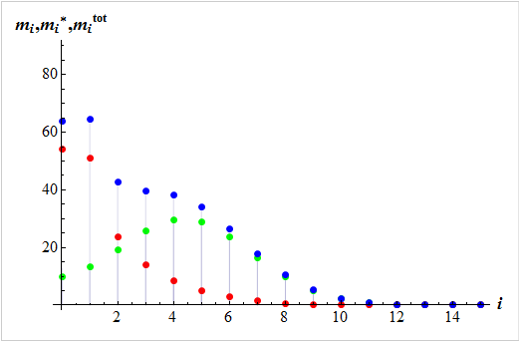
\includegraphics[width=\textwidth]{Images/ex_disc_eq}
\caption{Discrete model solutions}
\end{subfigure}
\begin{subfigure}[ht]{0.4\textwidth}
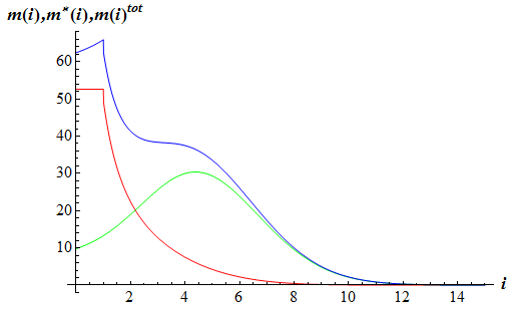
\includegraphics[width=\textwidth]{Images/ex_cont_eq}
\caption{Continuous approximation model solutions}
\end{subfigure}
\caption{Model results for parameters: $\imax=30,\lambda=5.4,\kappa 0=0.66,\tau 0=0.1,\mu 0=0.0292,\delta=0.1$}
\end{figure}

\begin{figure}[ht]
\centering
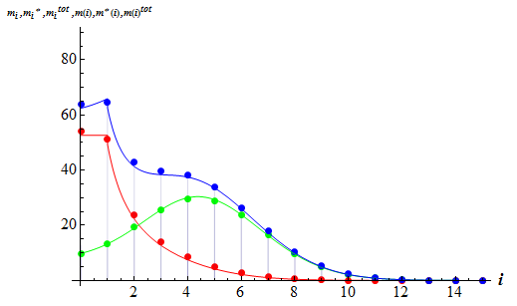
\includegraphics[width=\textwidth]{Images/ex_both_eq}
\caption{Comparison of discrete and continuous approximation model Solutions for Parameters: $\imax=30,\lambda=5.4,\kappa 0=0.66,\tau 0=0.1,\mu 0=0.0292,\delta=0.1$}
%\centering Red: Marked class, Green: Unmarked class, Blue: Total= unmarked+marked classes}
\end{figure}

Although solutions for only one set of parameter values is shown, the same behavior has been observed for all sets of parameters simulated.
Additionally, since the two solution were derived using different methods, they serve to validate each other.
Possessing two different methods to generate equilibrium distributions for the polysomal classes is advantageous in that it provides flexibility to researchers for model fitting and parameter estimation when investigating empirically derived data.

\section*{Additional Notes}
\subsection*{Getting Rid of GCD function}
If equation
\begin{equation}\label{eq:anyl_unmarked_imax}
m_{i_{max}}^{eq}=\dfrac{\prod_{i=1}^{i_{max}}\left(\frac{i}{GCD[i_{max},i]}\kappa_0\right)}{\prod_{i=1}^{i_{max}}\left(\frac{i_{max}}{GCD[i_{max},i]}(\mu_0+i\tau_0)+\frac{i}{GCD[i_{max},i]}\kappa_0\right)},
\end{equation}
 in previous versions of the write up is correct, then it seems we've missed a very simplification that would simplify our calculations \emph{immensely}.
Let's imagine three generic functions of $i$, $a_i$, $b_i$, and $c_i$ such that
\begin{align}
  F &= \frac{ \prod_i \left(a_i b_i\right)}{\prod_i \left(a_i c_i + a_i b_i\right)}\\
\intertext{Based on my understanding of mathematics,}
  F &= \frac{ \prod_i a_i \prod_i b_i }{\prod_i \left(a_i \left(c_i + b_i\right)\right)}\\
  &= \frac{ \prod_i a_i \prod_i b_i }{\prod_i a_i \prod_i \left(c_i + b_i\right)}\\
  &= \frac{\prod_i b_i }{\prod_i \left(c_i + b_i\right)}\\
\end{align}
If this is correct and we define $a_i = 1/\GCD[\imax, i]$ and $b_i \kappa_0$ and $c_i (\mu_0 + i \tau_0)$, then the equation \ref{eq:anyl_unmarked_imax} can be rewritten as,
\begin{equation}
  \hat{m}_{\imax}= \frac{ prod_{i=1}^{\imax} i \frac{\kappa_0}{\imax}}{prod_{i=1}^{\imax} \mu_0 + i \left(\tau_0 +\frac{\kappa_0}{\imax}\right)} 
\end{equation}
If this is the case, then I'm both elated and embarrassed as hell we didn't see it earlier.


%
%\newpage
%
%\part{Interpreting Data and Mapping the Model to Experimental Data}
%
%
%%\section{Determination of Solutions at Steady-State in Both the Continuous
%%and Discrete Models}
%
%%({*}{*} This should include some of the writing above, including the
%%techniques discussed that utilized the tridiagonal form of the matrix
%%and also using the determinant-adjoint technique for inverting the
%%matrix. {*}{*})
%
%
%\section{Interpreting Experimental Data}
%
%This section will discuss the technique used to interpret the experimental
%data for the distribution of polysomes.  The data being considered here is the work of \emph{J. Guan,} and \emph{A. VonArnim , University of Tennesse - Knoxville}.
%
%
%\subsection{Absorbance Data}
%
%Absorbance data has been generated by a variety of researchers to
%quantify the abundance of different classes of polysomes. This data is often broken down into polysomal
%fractions. The number of fractions can vary depending on the researcher;
%10 to 12 fractions is fairly common in the literature. It is also
%customary to lump the first fractions together into a single non-polysomal
%class. This class includes bare mRNA, those that have ribosomes still
%in the process of binding completely for translation, and those that
%have a single ribosome bound. This non-polysomal class can have up
%to four fractions included in it. A similiar phenonmenon takes place
%in the final fractions. Theoretically, the maximum number of ribosomes
%that can be bound is related to the length of the mRNA. This means
%there can be upwards of forty different mRNA classes (this number
%is related to \imax in the discrete model and $n$ in the continuous
%model). So with 12 fractions and 40 mRNA classes, there is necessarily
%an overlap of classes in each fraction.
%
%The absorbance data itself is reported as a the $log_{2}$ of integral
%of absorbance in each fraction.
%
%
%\subsection{Data Interpretation Techniques}
%
%In interpreting the data there are multiple elements that need to
%be considered first before the abundances estimated by the model can
%be matched up with the UV profiles. A function to relate mRNA class
%to the mean distance travelled in the profile is one piece of information
%that is needed. Also, an estimate of the variance in this travel distance
%is also needed. If a function is to be written to estimate these values,
%one must also know the total length of the UV-Profile, and the background,
%or baseline, amount of fluoresence.
%
%
%\subsubsection{Assumption of Normality and Determiniation of Distribution Parameters}
%
%If we assume that the distribution of mRNA of a given class in the
%UV profile is normally distributed with mean $\mu$and variance $\sigma$,
%then there are graphical techniques that can be used to determine
%these constants directly from UV-Profile diagrams.
%
%Mean distance traveled in the UV Profile is estimated by measuring
%the distance of the peaks in the profile from the ``origin'' in
%the profile (where the origin represents 0\% absorbance and 0 distance
%travelled). This was done by importing the PDF image of the UV-Profile
%into \emph{Mathematica} and then using the standard \emph{'get-coordinates'}
%graphing tool. This work took place under the asssumption that the
%first visible peak in the UV-Profile was from the mRNA class with
%2 ribosomes bound. The coordinates of each distinguishable peak thereafter
%was also found and this data was used to fit a saturating function
%whose maximum value was given by the total length of the UV-Profile.
%The function fitting was performed in \emph{Mathematica }using \emph{'FindFit'}.
%
%The variance was determined by gathering points from the different
%peaks and utilizing the property of the Normal distribution that the
%2nd derivative is related to the curvature of the function. A quadratic
%function was fit to each peak and then the second deriative was found
%and equated to the second derivative of the probability distribution
%function of the Normal distribution. In this way, the distribution
%parameter $\sigma$ was able to be found. Then with estimates of $\sigma$from
%each distinguishable peak in the profile, a function was fit in order
%to estimate $\sigma$ as function of the polysomal class.
%
%Using the estimated values for mean and variance, denoted $\mu_{est}(i)$
%and $\sigma_{est}(i)$ respectively, a mixed PDF was created to mimic
%the UV-Profile. The mixed PDF is comprised of the normal distributions
%$N_{i}(\mu_{est}(i),\sigma_{est}(i))$ and is denoted as $M_{pdf}(N_{i}).$
%
%
%\subsubsection{Connecting the Model to Absorbance Data}
%
%With a function created to mimic the UV-Profile image, the next step
%is to use the absorbance Data to estimate parameters in the model.
%The assumption is made that the height of each peak (and necessarily
%the $log_{2}$of the integral in a fraction) in the UV-Profile is
%proportional to the abundance of each polysomal class. The distribution
%of these abundances is what the model predicts, and so within the
%model we see that the fluoresence in a fraction can be viewed as a
%function of the model parameters and the distribution parameters.
%Letting $\Lambda$represent the vector of model parameters, and $Y_{j}$
%represent the measured absorbance data in fraction $j,$we have
%the following relationship:
%\[
%Y_{j}\propto log_{2}(\sum_{i}\int_{j}^{j+1}m_{tot}(i,\Lambda)\, N_{i}(\mu_{est}(i),\sigma_{est}(i))di)
%\]
%
%
%This states that the amount of absorbance in fraction $j$ is proportional
%to the integral of each Normal function on that fraction times the
%abundance calculated from the model, since each normal function is
%not isolated completely to a fraction, we need to sum the contributions
%from all the functions, which is why the summation over all values
%of $i$ is needed in the relationship. This proportionality is lays
%the framework for the minimization and estimation of the model parameters,
%$\Lambda.$
%
%
%\subsection{Minimization for Parameter Estimation}
%
%This section will present the motivation for the minimization technique
%utilized in the research thusfar. Based on the assumption of Normally
%distributed error (or noise) in the measurement, minimization of the
%sums of difference in model predictions and measurement squared is
%used. This method maximizes Log-Likelihood for the parameter estimates.
 %
%
%
%\subsubsection{Minimization Scheme}
%
%Definitions of the functions and variables used will be given below.
%Beginning with the definitions and relationship relating the data
%to the model estimations in a fluorsecence fraction, where $j\in J$:
%\begin{description}
%\item [{$f_{j}$:}] True value of absorbance in $j^{th}$ fraction, without
%noise in measurement. This is related to model estimates. When considering
%model estimates of this, it will be written as $(f_{j}|\Lambda)$
%\item [{$F_{j}$:}] Value of absorbance in $j^{th}$ fraction with noise
%added.
%\item [{$\epsilon$:}] The amount measurement error or noise, the difference
%between $f_{j}$ and $F_{j}$
%\end{description}
%Related by the following, under the assumption that the noise in each
%fraction has the same distribution:
%
%\begin{align*}
%F_{j} &= f_{j}\cdot\hat{\epsilon}\\
%log_{2}(F_{j}) &= log_{2}(f_{j})+log_{2}(\hat{\epsilon})\\
%Where & \, & \hat{\epsilon}\sim N(0,\sigma_{\epsilon})
%\end{align*}
%The data being considered is given in $log_{2}$of the absorbance
%in a fraction, so for convenience the following will be used:
%\begin{description}
%\item $G_{j}=Log_{2}(F_{j})$
%\item $g_{j}=Log_{2}(f_{j})$
%\item $\epsilon=Log_{2}(\hat{e})\sim LogNormal(0,\sigma_{\epsilon})$
%\end{description}
%Then, the likelihood of $G_{j}$, is given by the following:
%\begin{align*}
%Lik(G_{j}) &= \dfrac{1}{\sqrt{2\pi\sigma_{\epsilon}}}Exp(-\dfrac{(G_{j}-(g_{j}|\Lambda))^{2}}{2\sigma_{\epsilon}^{2}})
%\end{align*}
%
%
%and the $negative\; loglikelihood$ is given by:
%\begin{equation*}
%-LLik(G_{j})=-\ln(\dfrac{1}{\sqrt{2\pi}})+\ln(\sigma_{\epsilon})+\dfrac{(G_{j}-(g_{j}|\Lambda))^{2}}{2\sigma_{\epsilon}^{2}}
%\end{equation*}
%
%
%The objective function to minimize is then:
%\begin{equation*}
%\min_{j}\; n\ln(\sigma_{\epsilon})+\sum_{j\in J}\dfrac{(G_{j}-(g_{i}|\Lambda))^{2}}{2\sigma_{\epsilon}^{2}}
%\end{equation*}
%
%\section{Results}
%
%This section will include our results from simulation as they become available.
%\part*{Appendix}
%\section*{A1: Example solutions to unmarked system for ODE formulation at equilibrium}
%\begin{description}
%\item This set of solutions is generated from solving the system of unmarked ODE at equilibrium directly using \emph{Solve[]} in \emph{Mathematica}
%\item For $\imax=1$
%\item \hspace{5pt} $\left\{M(0)\to \frac{\lambda  (\mu +\tau )}{\mu  (\kappa +\mu +\tau )},M(1)\to \frac{\kappa  \lambda }{\mu  (\kappa +\mu +\tau )}\right\}$
%\item For $\imax=2$ 
%\item \hspace{5pt} $\left\{M(0)\to \frac{\lambda  (\kappa  \mu +(\mu +\tau ) (\mu +2 \tau ))}{\mu  \left(\kappa ^2+2 \kappa  (\mu +\tau )+(\mu +\tau ) (\mu +2 \tau )\right)},M(1)\to \frac{\kappa  \lambda  (\mu +2 \tau )}{\mu  \left(\kappa ^2+2 \kappa  (\mu +\tau )+(\mu +\tau ) (\mu +2 \tau )\right)},M(2)\to \frac{\kappa ^2 \lambda }{\mu  \left(\kappa ^2+2 \kappa  (\mu +\tau )+(\mu +\tau ) (\mu +2 \tau )\right)}\right\}$ 
%\item For $\imax=3$
%\item \hspace{5pt} $\Big\{ M(0)\to \frac{\lambda  \left(\kappa ^2 \mu +2 \kappa  \mu  (\mu +2 \tau )+(\mu +\tau ) (\mu +2 \tau ) (\mu +3 \tau )\right)}{\mu  \left(\tau ^2 (6 \kappa +11 \mu )+3 \tau  (\kappa +2 \mu ) (\kappa +\mu )+(\kappa +\mu )^3+6 \tau ^3\right)},M(1)\to \frac{\kappa  \lambda  (\kappa  \mu +(\mu +2 \tau ) (\mu +3 \tau ))}{\mu  \left(\tau ^2 (6 \kappa +11 \mu )+3 \tau  (\kappa +2 \mu ) (\kappa +\mu )+(\kappa +\mu )^3+6 \tau ^3\right)},$
%\item \hspace{9pt} $ M(2)\to \frac{\kappa ^2 \lambda  (\mu +3 \tau )}{\mu  \left(\tau ^2 (6 \kappa +11 \mu )+3 \tau  (\kappa +2 \mu ) (\kappa +\mu )+(\kappa +\mu )^3+6 \tau ^3\right)},M(3)\to \frac{\kappa ^3 \lambda }{\mu  \left(\tau ^2 (6 \kappa +11 \mu )+3 \tau  (\kappa +2 \mu ) (\kappa +\mu )+(\kappa +\mu )^3+6 \tau ^3\right)} \Big\} $
%\item For $\imax=4$
%\item \hspace{5pt} $\Big\{M(0)\to \frac{\lambda  \left(\mu  \tau ^2 (18 \kappa +35 \mu )+5 \mu  \tau  (\kappa +\mu ) (\kappa +2 \mu )+\mu  (\kappa +\mu )^3+50 \mu  \tau ^3+24 \tau ^4\right)}{\mu  \left(2 \tau ^3 (12 \kappa +25 \mu )+\tau ^2 (2 \kappa +5 \mu ) (6 \kappa +7 \mu )+2 \tau  (2 \kappa +5 \mu ) (\kappa +\mu )^2+(\kappa +\mu )^4+24 \tau ^4\right)},$
%\item \hspace{9pt} $M(1)\to \frac{\kappa  \lambda  \left(\kappa ^2 \mu +2 \kappa  \mu  (\mu +3 \tau )+(\mu +2 \tau ) (\mu +3 \tau ) (\mu +4 \tau )\right)}{\mu  \left(2 \tau ^3 (12 \kappa +25 \mu )+\tau ^2 (2 \kappa +5 \mu ) (6 \kappa +7 \mu )+2 \tau  (2 \kappa +5 \mu ) (\kappa +\mu )^2+(\kappa +\mu )^4+24 \tau ^4\right)},$
%\item \hspace{9pt} $M(2)\to \frac{\kappa ^2 \lambda  (\kappa  \mu +(\mu +3 \tau ) (\mu +4 \tau ))}{\mu  \left(2 \tau ^3 (12 \kappa +25 \mu )+\tau ^2 (2 \kappa +5 \mu ) (6 \kappa +7 \mu )+2 \tau  (2 \kappa +5 \mu ) (\kappa +\mu )^2+(\kappa +\mu )^4+24 \tau ^4\right)},$\item \hspace{9pt} $M(3)\to \frac{\kappa ^3 \lambda  (\mu +4 \tau )}{\mu  \left(2 \tau ^3 (12 \kappa +25 \mu )+\tau ^2 (2 \kappa +5 \mu ) (6 \kappa +7 \mu )+2 \tau  (2 \kappa +5 \mu ) (\kappa +\mu )^2+(\kappa +\mu )^4+24 \tau ^4\right)},$
%\item \hspace{9pt} $M(4)\to \frac{\kappa ^4 \lambda }{\mu  \left(2 \tau ^3 (12 \kappa +25 \mu )+\tau ^2 (2 \kappa +5 \mu ) (6 \kappa +7 \mu )+2 \tau  (2 \kappa +5 \mu ) (\kappa +\mu )^2+(\kappa +\mu )^4+24 \tau ^4\right)}\Big\}$
%
%\item Recall that the marked solutions are solved completely in terms of the unmarked solutions using equation (7).
%
%\end{description}

\end{document}
